\newpage
\section{Redes Neuronales}

\noindent Las redes neuronales artificiales, son un algoritmo basado en el funcionamiento de las propias neuronas del cerebro que reciben señales de entradas de las neuronas con las cuales están conectadas, las procesan y envían el resultado a las neuronas con las que estén conectadas. 

\noindent El algoritmo de aprendizaje que oculta una red neuronal es la optimización de algún funcional, de manera que estas se pueden aplicar a problemas que consistan en la resolución de dichos problemas. La ventaja de este tipo de algoritmos es que en esencia, son un conjunto de parámetros que pueden ser ajustados para cualquier tarea y cualquier tipo de función a aproximar solo hace falta la complejidad del modelo adecuada según \emph{Hornik, K., Stinchcombe, M., y  White, H.} \cite{Hornik 1989}.  

\noindent Una neurona artificial es mucho más simple que una neurona, \emph{López R., E. Balsa-Canto y E. Oñate} \cite{Roberto 2008} definen una neurona en términos matemáticos , pero antes hay que definir los siguientes conceptos.

\noindent Sea un vector aleatorio $\mathbf{x}$ de longitud $p$, llamamos datos de entrada a los números que se introducen en la neurona que pueden ser los propios valores observados de las 
\begin{defi}
Llamaremos \emph{pesos sinápticos} $\omega$ de una neurona, al vector de $p$ constantes que regulan la importancia de cada entrada en la neurona.  A este vector de pesos sinápticos se le puede añadir un término independiente que únicamente se sumará, se le llama \emph{sesgo} y se denota como $b$.
\end{defi}

\begin{defi}
Se llama \emph{función de activación}, $f$ de una neurona artificial a la función que transforma la suma ponderada de las entradas para obtener la salida. 

\noindent Las funciones de activación más habituales son; la función \emph{identidad} \emph{En este caso es como si se hiciera una simple suma ponderada de los datos de entrada}, la función \emph{sigmoide}, la \emph{tangente hiperbólica} o la función \emph{lineal regularizada} para casos de regresión, es decir, en casos en los que la variable respuesta sea continua. En caso contrario, se pueden utilizar la \emph{función softmax} o la \emph{función de regresión logística} para casos discretos, ya que devuelven valores en el intervalo $[0,1]$ y se puede asociar con la probabilidad de pertenecer a una clase u otra. 
\end{defi}
\begin{defi}
Una neurona procesa una entrada $\textbf{x}$ de acuerdo con unos \emph{pesos sinápticos} $(b,\omega)$ que luego es transformada por una función de activación $g(u)$, las más habituales son la función sigmoide, una función lineal, la tangente hiperbólica o directamente la identidad. 

\noindent Una  vez definidos los elementos que forman una neurona artificial estos se utilizan de manera que se utiliza la función:
\begin{equation}
\begin{split}
f:\mathbb{R}^p &\longrightarrow \mathbb{R}\\
f(\textbf{x})&\longrightarrow f(\textbf{x};b,\omega)
\end{split}
\end{equation}

\begin{equation}
f(\textbf{x})=g\left(b+\sum_{i=1}^p \omega_i x_i\right)
\end{equation}
El siguiente diagrama proporciona una forma sencilla de entender el funcionamiento de dicho modelo, incluyendo la analogía de las neuronas biológicas. 
\end{defi}
\begin{center}
%%Hay que pedirle a Carlos que lo edite por que yo la verdad que no se 
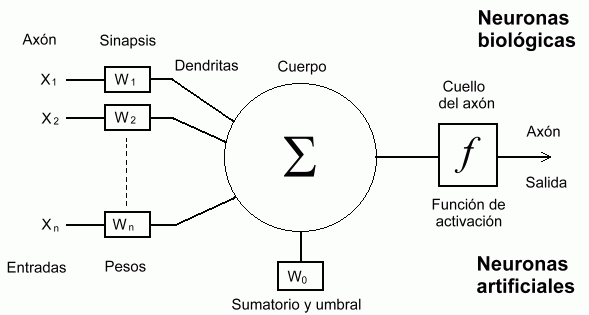
\includegraphics[scale=0.6]{Documentos Extra/Imagenes/neurona.png}
\end{center}

\noindent La principal ventaja de estos métodos es que las neuronas se pueden conectar entre ellas, es decir, estas se pueden organizar de manera que los datos de salida de un conjunto de neuronas sirvan como entrada del siguiente.
\begin{defi}
Se llama \emph{capa de neuronas} al conjunto de neuronas artificiales que tienen el mismo conjunto de datos de entrada y cuyos datos de salida para la siguiente.
\end{defi}

\noindent Se pueden establecer varios tipos de capas de neuronas \cite{Neural Designer}:
\begin{defi}
Se llama \emph{capa de entrada} a la primera capa de neuronas que recibe los valores de las observaciones y las estandariza (\emph{Se debe entrenar al modelo para ello}). Se establece una 
\end{defi}

\begin{defi}
Se llama \emph{capa oculta} a cada una de las capas intermedias que se utilizan en las redes neuronales. 
\end{defi}

\begin{defi}
Se llama \emph{capa de salida} a la última capa que tiene tantas neuronas como variables respuesta y sus datos de salida son las predicciones de 
\end{defi}

\noindent Para el proceso de ajuste se utiliza de manera habitual el método del gradiente con un conjunto de datos con $N$ observaciones. En el capitulo  11 \emph{Hastie et.al. }\cite{Hastie 2001} se detallan en profundidad el ajuste mediante el método del gradiente. De esta manera, se tiene un proceso que se llama \emph{back-propagation}. 

\noindent La siguiente imagen es un esquema de una red neuronal con 7 capas de neuronas interconectadas donde la primera capa es de escalado y la última de desescalado. Se puede observar que se predicen las variables $y_1, y_2, y_3$ usando como entrada las variables $x_1,x_2,x_3,x_4$ 

\begin{figure}[h]
\centering
%%Hay que pedirle a Carlos que lo edite por que yo la verdad que no se 
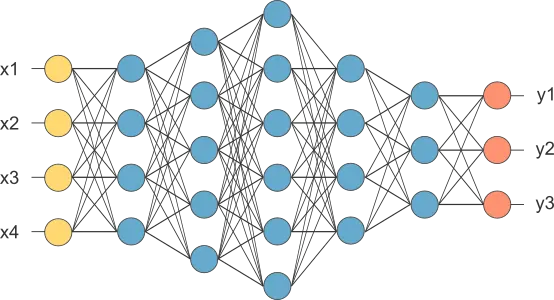
\includegraphics[scale=0.35]{Documentos Extra/Imagenes/red-neuronal-grande.png}
\caption{Imagen extraída directamente de www.neuraldesigner.com}
\end{figure}

\noindent Si se quisiera expresar el modelo como una única expresión, la expresión que se obtiene al hacer crecer un poco la red neuronal es bastante compleja de interpretar, por ejemplo en el caso anterior se tiene más de 100 parámetros y no es una red demasiado compleja, por tanto la interpretación del modelo es compleja. Es por ello, que las redes neuronales se utilizan únicamente para fines predictivos \cite{Hastie 2001, James 2013}. 

\noindent Las principales ventajas es que estos modelos pueden ajustarse a datos no lineales sin saber a priori que tipo de no linealidad se tiene. Por otro lado, debido a la gran cantidad de parámetros a ajustar pueden provocar \emph{sobre-ajuste} pero para ello se pueden utilizar técnicas de validación cruzada \emph{(Capítulo 5 de \cite{James 2013} o el capítulo 7 de \cite{Hastie 2001})}

\noindent En esta memoria se han detallado los tipos más básicos de neuronas hay tareas específicas que este tipo de neuronas no pueden afrontar, por ejemplo, en el caso de datos que proceden de series temporales en las que estados previos influyen en los estados futuros como puede ser predicciones meteorológicas, bursátiles etc... se han desarrollado un tipo más complejo de neuronas llamadas LSTM \emph{(Long-Short Term Memory)} de las que se puede ver su desarrollo y definición además de las propiedades que poseen en \cite{Hochreiter 1997}. \emph{(Para una descripción más esquemática véase \cite{Neural Designer})}

